\documentclass[12pt]{article}
\usepackage{amsmath, amssymb, amsfonts, amsthm, mathtools, relsize}
\DeclarePairedDelimiter\ceil{\lceil}{\rceil}
\DeclarePairedDelimiter\floor{\lfloor}{\rfloor}
\usepackage{thmtools}
\usepackage[utf8]{inputenc}
\usepackage[inline]{enumitem}
\usepackage{graphicx, wrapfig, float}
\usepackage[colorlinks=true]{hyperref}
\setlength\parindent{0pt}

\theoremstyle{definition}
\newtheorem{thm}{Theorem}
\numberwithin{thm}{section}
\newtheorem{lem}[thm]{Lemma}
\newtheorem{defn}[thm]{Definition}
\newtheorem{prop}[thm]{Proposition}
\newtheorem{cor}[thm]{Corollary}
\newtheorem{ex}{Example}


\let\emptyset\varnothing
\newcommand{\id}{\operatorname{id}}
\newcommand{\hint}[1]{\textbf{HIDDEN:} {\color[rgb]{0.95, 0.95, 0.95}#1}}

\pagestyle{plain}

\usepackage{titlesec}
\titleformat{\section}[block]{\sffamily\Large\filcenter\bfseries}{\S\thesection.}{0.25cm}{\Large}
\titleformat{\subsection}[block]{\large\bfseries\sffamily}{\S\S\thesubsection.}{0.2cm}{\large}

\usepackage[a4paper]{geometry}
\usepackage{lipsum}

\usepackage{cleveref}
\crefname{thm}{Theorem}{Theorems}
\crefname{lem}{Lemma}{Lemmas}
\crefname{defn}{Definition}{Definitions}
\crefname{prop}{Proposition}{Propositions}
\crefname{cor}{Corollary}{Corollaries}
\crefname{equation}{}{}

\usepackage{mdframed}
\newenvironment{blockquote}
{\begin{mdframed}[skipabove=0pt, skipbelow=0pt, innertopmargin=4pt, innerbottommargin=4pt, bottomline=false,topline=false,rightline=false, linewidth=2pt]}
{\end{mdframed}}
\newenvironment{soln}{\begin{proof}[Solution]}{\end{proof}}

\usepackage{titlesec}
\titleformat{\section}[block]{\sffamily\Large\filcenter\bfseries}{\S\thesection.}{0.25cm}{\Large}
\titleformat{\subsection}[block]{\large\bfseries\sffamily}{\S\S\thesubsection.}{0.2cm}{\large}

\usepackage{fancyhdr}
\pagestyle{fancy}
\fancyhf{}
\fancyhead[L]{\sffamily{\S\textbf{\nouppercase{\leftmark}}}}
\fancyhead[R]{\sffamily{\thepage}}

\renewcommand{\familydefault}{\sfdefault}

\title{CS 736: Medical Image Computing\\\large{Assignment 1}}
\author{Siddharth Khandelwal - 190070062\\Prasann Viswanathan - 190070047}
\date{Spring 2020-21}

\begin{document}
\maketitle
\tableofcontents
\listoffigures
\newpage
\section{Question 1}
\begin{enumerate}[label=(\alph*)]
\item The RRMSE value between the noisy and noiseless images is 0.2986
\item Different parameter and RRMSE values for the applied priors are:
\begin{enumerate}[label=(\arabic*)]
\item MRF Prior: Quadratic Model-
	\begin{enumerate}
		\item $\alpha$=0.29 
		\item RRMSE($\alpha$)=0.26669
		\item RRMSE(1.2$\alpha$)=0.26911
		\item RRMSE(0.8$\alpha$)=0.28746
	\end{enumerate}
	\item MRF Prior: Discontinuity-adaptive Huber function-
	\begin{enumerate}
		\item $\alpha$=0.01
		\item $\gamma$=0.68 
		\item RRMSE($\alpha$, $\gamma$)=0.27816
		\item RRMSE(1.2$\alpha$, $\gamma$)=0.27788
		\item RRMSE(0.8$\alpha$, $\gamma$)=0.27843
		\item RRMSE($\alpha$, 1.2$\gamma$)=0.27829
		\item RRMSE($\alpha$, 0.8$\gamma$)=0.27820
	\end{enumerate}
	\item MRF Prior: Discontinuity-adaptive function-
	\begin{enumerate}
		\item $\alpha$=0.01 
		\item $\gamma$=0.01
		\item RRMSE($\alpha$, $\gamma$)=0.27947
		\item RRMSE(1.2$\alpha$, $\gamma$)=0.27945
		\item RRMSE(0.8$\alpha$, $\gamma$)=0.27948
		\item RRMSE($\alpha$, 1.2$\gamma$)=0.27948
		\item RRMSE($\alpha$, 0.8$\gamma$)=0.27945
	\end{enumerate}
\end{enumerate} \newpage
\item Images expressed as color jetmap:
	\begin{figure}[H]
		\centering
    	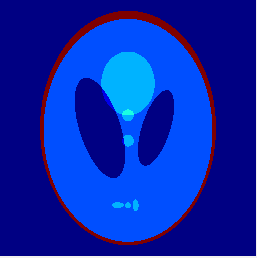
\includegraphics[width=0.55\textwidth]{imgs/Original_Phantom.png}
    	\caption{Noiseless Image (Phantom)}
    	\label{fig:NL1}
	\end{figure}
	\begin{figure}[H]
		\centering
    	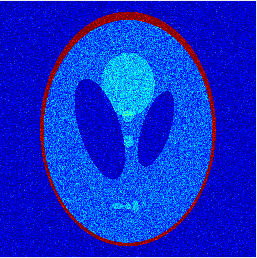
\includegraphics[width=0.55\textwidth]{imgs/Noisy_Phantom.png}
    	\caption{Noisy Image (Phantom)}
    	\label{fig:N1}
	\end{figure}
	\begin{figure}[H]
		\centering
    	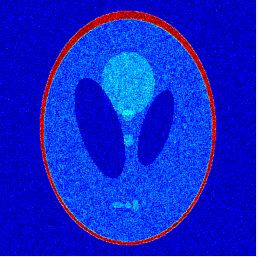
\includegraphics[width=0.55\textwidth]{imgs/Quadratic_Phantom.png}
    	\caption{MRF Prior: Quadratic (Phantom)}
    	\label{fig:Q1}
	\end{figure}
	\begin{figure}[H]
		\centering
    	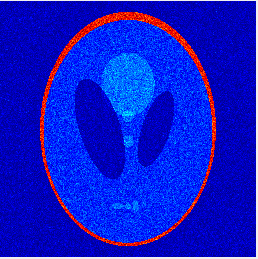
\includegraphics[width=0.55\textwidth]{imgs/DAH_Phantom.png}
    	\caption{MRF Prior: Discontinuity-adaptive Huber (Phantom)}
    	\label{fig:DAH1}
	\end{figure}
	\begin{figure}[H]
		\centering
    	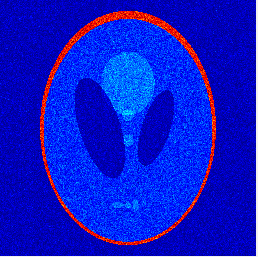
\includegraphics[width=0.55\textwidth]{imgs/DA_Phantom.png}
    	\caption{MRF Prior: Discontinuity-adaptive (Phantom)}
    	\label{fig:DA1}
	\end{figure}
\item Plots of RRMSE vs iteration:
	\begin{figure}[H]
		\centering
    	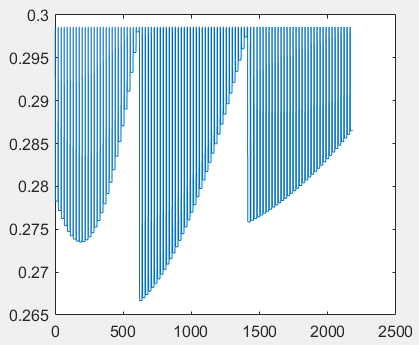
\includegraphics[width=0.55\textwidth]{imgs/Quadratic_Phantom_RRMSE.png}
    	\caption{MRF Prior: Quadratic (Phantom)}
    	\label{fig:Q1G}
	\end{figure}
	\begin{figure}[H]
		\centering
    	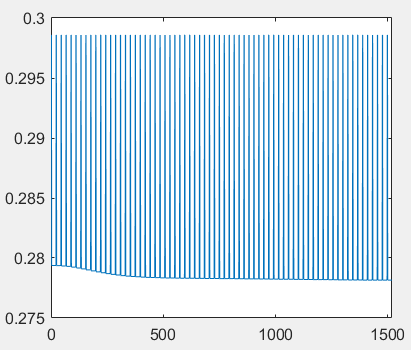
\includegraphics[width=0.55\textwidth]{imgs/DAH_Phantom_RRMSE.png}
    	\caption{MRF Prior: Discontinuity-adaptive Huber (Phantom)}
    	\label{fig:DAH1G}
	\end{figure}
	\begin{figure}[H]
		\centering
    	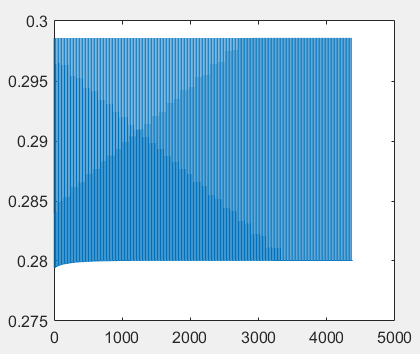
\includegraphics[width=0.55\textwidth]{imgs/DA_Phantom_RRMSE.png}
    	\caption{MRF Prior: Discontinuity-adaptive (Phantom)}
    	\label{fig:DA1G}
	\end{figure}
\end{enumerate}
\newpage

\section{Question 2}
\begin{enumerate}[label=(\alph*)]
\item The RRMSE value between the noisy and noiseless images is 0.14245
\item Different parameter and RRMSE values for the applied priors are:
\begin{enumerate}[label=(\arabic*)]
\item MRF Prior: Quadratic Model-
	\begin{enumerate}
		\item $\alpha$=0.82 
		\item RRMSE($\alpha$)=0.11925
		\item RRMSE(1.2$\alpha$)=0.12070
		\item RRMSE(0.8$\alpha$)=0.13245
	\end{enumerate}
	\item MRF Prior: Discontinuity-adaptive Huber function-
	\begin{enumerate}
		\item $\alpha$=0.01
		\item $\gamma$=0.69 
		\item RRMSE($\alpha$, $\gamma$)=0.14092
		\item RRMSE(1.2$\alpha$, $\gamma$)=0.14086
		\item RRMSE(0.8$\alpha$, $\gamma$)=0.14097
		\item RRMSE($\alpha$, 1.2$\gamma$)=0.14092
		\item RRMSE($\alpha$, 0.8$\gamma$)=0.14092
	\end{enumerate}
	\item MRF Prior: Discontinuity-adaptive function-
	\begin{enumerate}
		\item $\alpha$=0.01 
		\item $\gamma$=0.01
		\item RRMSE($\alpha$, $\gamma$)=0.14116
		\item RRMSE(1.2$\alpha$, $\gamma$)=0.14115*
		\item RRMSE(0.8$\alpha$, $\gamma$)=0.14117
		\item RRMSE($\alpha$, 1.2$\gamma$)=0.14116
		\item RRMSE($\alpha$, 0.8$\gamma$)=0.14115*\\\\
		\hfill\small{* - Lesser RRMSE becausewell below the precision of our gamma steps}
	\end{enumerate}
\end{enumerate}\newpage
\item Images expressed as color jetmap:
	\begin{figure}[H]
		\centering
    	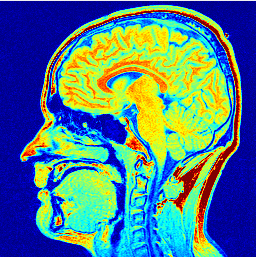
\includegraphics[width=0.55\textwidth]{imgs/Original_BrainMRI.png}
    	\caption{Noiseless Image (Brain MRI)}
    	\label{fig:NL2}
	\end{figure}
	\begin{figure}[H]
		\centering
    	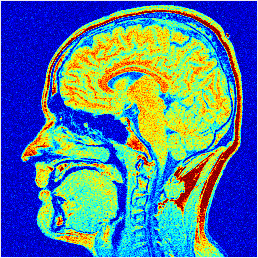
\includegraphics[width=0.55\textwidth]{imgs/Noisy_BrainMRI.png}
    	\caption{Noisy Image (Brain MRI)}
    	\label{fig:N2}
	\end{figure}
	\begin{figure}[H]
		\centering
    	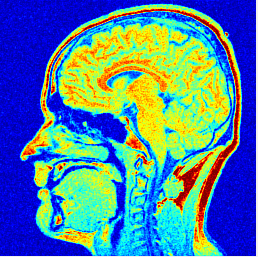
\includegraphics[width=0.55\textwidth]{imgs/Quadratic_BrainMRI.png}
    	\caption{MRF Prior: Quadratic (Brain MRI)}
    	\label{fig:Q2}
	\end{figure}
	\begin{figure}[H]
		\centering
    	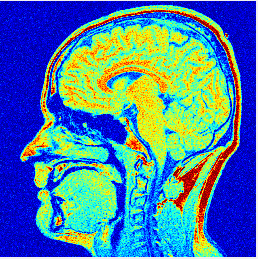
\includegraphics[width=0.55\textwidth]{imgs/DAH_BrainMRI.png}
    	\caption{MRF Prior: Discontinuity-adaptive Huber (Brain MRI)}
    	\label{fig:DAH2}
	\end{figure}
	\begin{figure}[H]
		\centering
    	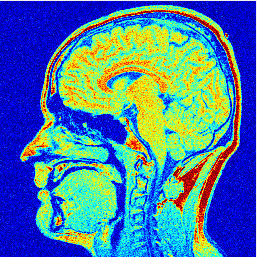
\includegraphics[width=0.55\textwidth]{imgs/DA_BrainMRI.png}
    	\caption{MRF Prior: Discontinuity-adaptive (Brain MRI)}
    	\label{fig:DA2}
	\end{figure}
\item Plots of RRMSE vs iteration:
	\begin{figure}[H]
		\centering
    	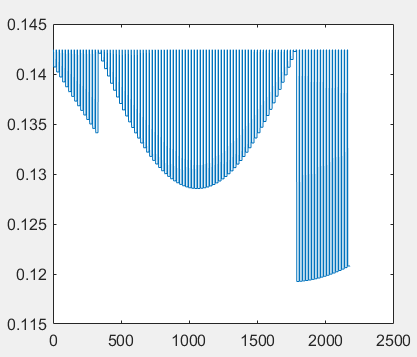
\includegraphics[width=0.55\textwidth]{imgs/Quadratic_BrainMRI_RRMSE.png}
    	\caption{MRF Prior: Quadratic (Brain MRI)}
    	\label{fig:Q2G}
	\end{figure}
	\begin{figure}[H]
		\centering
    	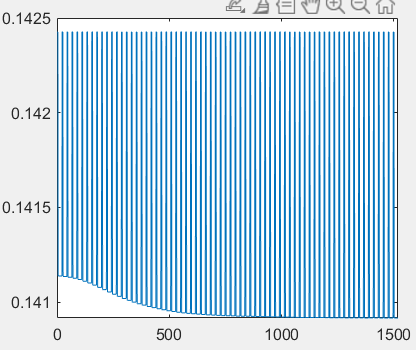
\includegraphics[width=0.55\textwidth]{imgs/DAH_BrainMRI_RRMSE.png}
    	\caption{MRF Prior: Discontinuity-adaptive Huber (Brain MRI)}
    	\label{fig:DAH2G}
	\end{figure}
	\begin{figure}[H]
		\centering
    	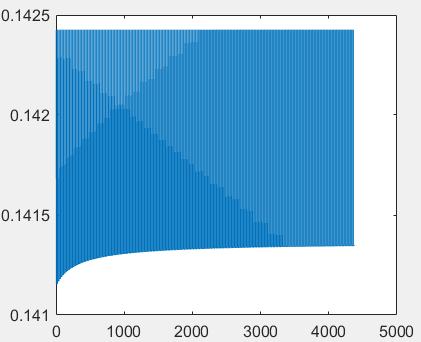
\includegraphics[width=0.55\textwidth]{imgs/DA_BrainMRI_RRMSE.png}
    	\caption{MRF Prior: Discontinuity-adaptive (Brain MRI)}
    	\label{fig:DA2G}
	\end{figure}
\end{enumerate}
\newpage
\section{Question 3}
\begin{enumerate}[label=(\alph*)]
\item A suitable MRF Prior for the coloured image with statistical dependency on RGB channels could be the Disconitnuity Adaptive Huber function coupled with a 6 neighbour neighbourhood system. We need a six neighbour system because the different colour channels are said to be statistically dependent on each other. \\
Also, RGB microscopy images have many discontinuities and outliers which is why a quadratic prior function wouldn't be ideal. \\
The updates to this will be performed in the same way using circshift but with additional shifts in the third dimension to account for added neighbors via coloured channels.
\item A suitable noise model is the poisson model as mentioned in the slides. Lambda shall be the true signal value and we will update using the corresponding cost function.
\item Using gradient descent updates we can do the same algorithm as black and white image. It shall be more computationally expensive. 
\end{enumerate}
\end{document}